\documentclass[a4paper]{article}


\usepackage[russian]{babel}
\usepackage[utf8]{inputenc}
\usepackage{graphicx}


\title{Лабораторная работа №3}
\author{Антипов Денис, гр. 5539 (вариант 17)}

\begin{document}
\maketitle

\section{Описание задачи}

Разработать эволюционный алгоритм, решающий задачу коммивояжера с помощью путевого представления. Для тестирования использовать координаты 29 городов в Западной Сахаре.

\section{Описани алгоритма}
\begin{itemize}
\item Варьируемые параметры алгоритма:
\begin{itemize}
\item Вероятность кроссинговера
\item Вероятность мутации
\item Размер популяции
\item Размер следующего поколения
\end{itemize}
\item Индивид представляется вектором, состоящим из номеров городов в порядке их обхода. Начальное поколение генерируется из случайных путей
\item Оператор редукции использует отбор с помощью рулетки (получилось быстрее турнирного отбора).
\item Для кроссинговера используются операторы PMX и OX. С CX не получилось, так как его описание в методичке слишком непонятная, а в интернете слишком мало информации о нем.
\item Оператор мутации случайным образом меняет местами два города в порядке обхода для каждого индивида из нового поколения с вероятностью мутации.
\item Новое поколение доукомплектовываается до размера популяции лучшими особями прошлого поколения.
\end{itemize}

\newpage
\section{Результаты работы алгоритма}

Несколько результатов для запуска с PMX (50 итераций): 

\begin{tabular}{cc}
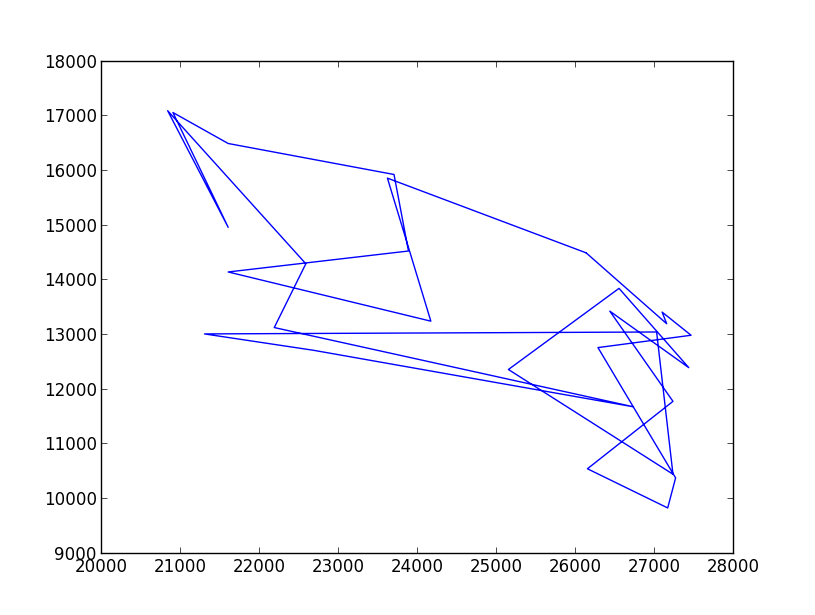
\includegraphics[width=7cm]{1.png} & 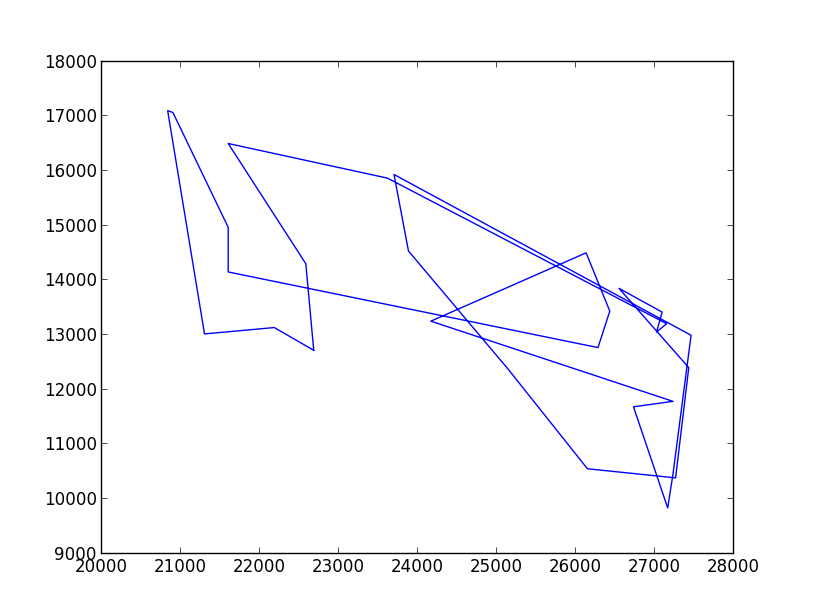
\includegraphics[width=7cm]{2.png} \\
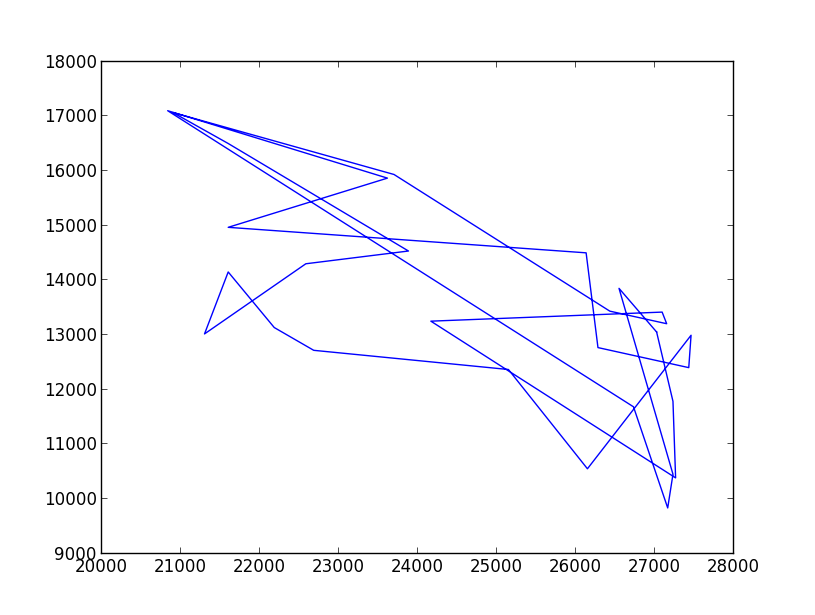
\includegraphics[width=7cm]{3.png} & 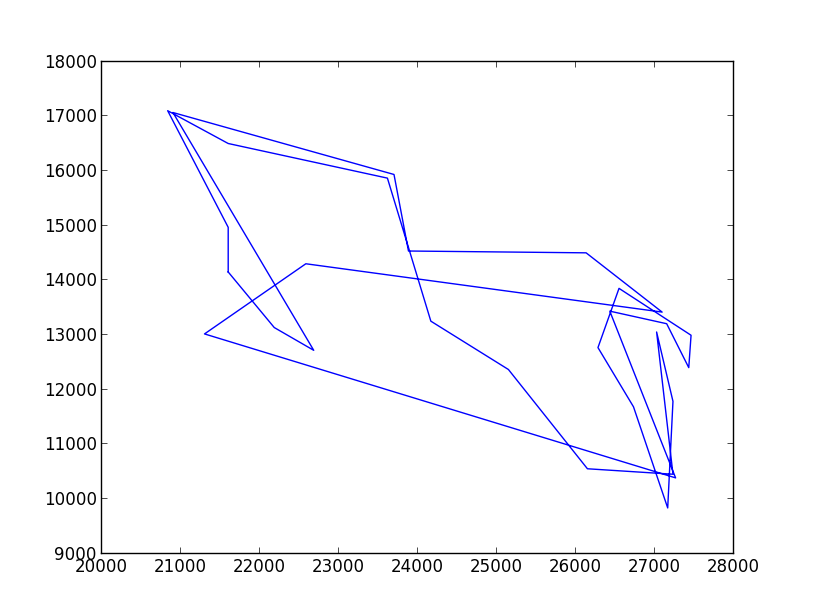
\includegraphics[width=7cm]{4.png}
\end{tabular}

\newpage
Результаты для OX:


\begin{tabular}{cc}
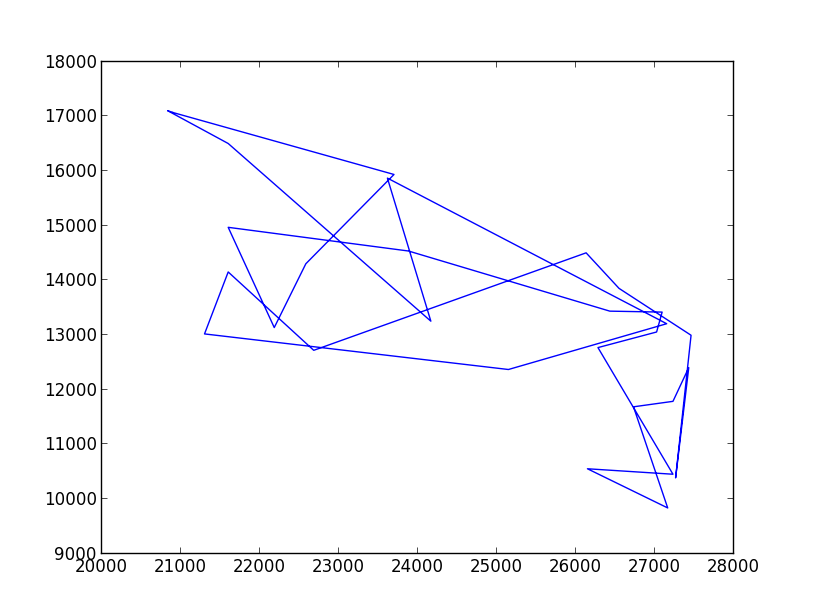
\includegraphics[width=7cm]{5.png} & 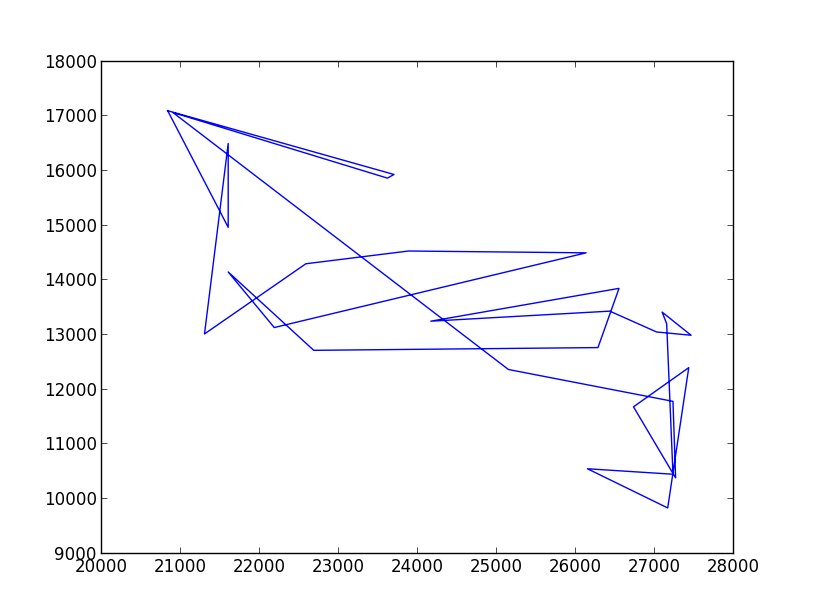
\includegraphics[width=7cm]{6.png} \\
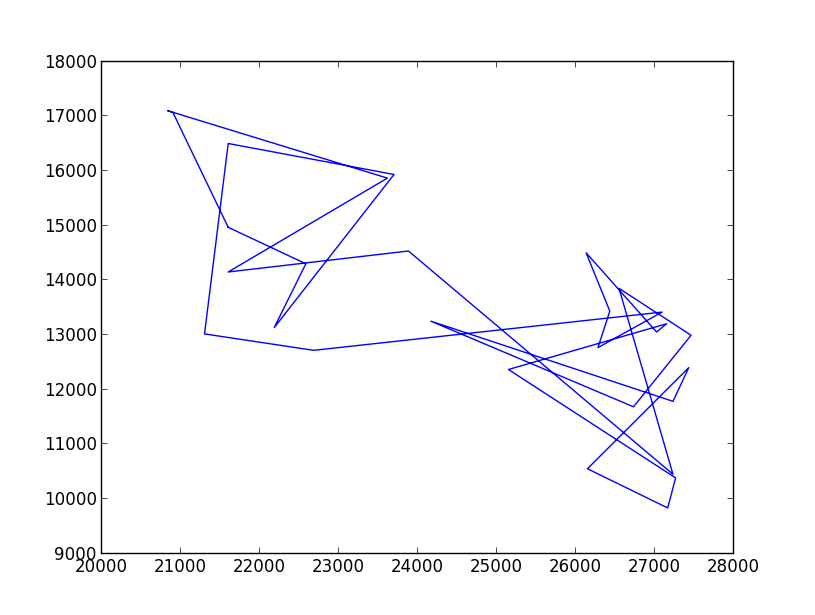
\includegraphics[width=7cm]{7.png} & 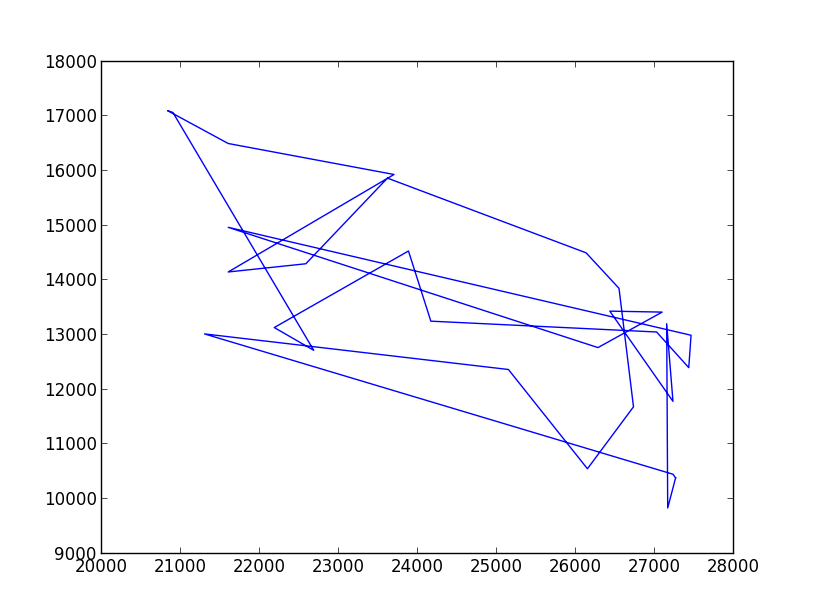
\includegraphics[width=7cm]{8.png}
\end{tabular}

Мы можем видеть, что результата за 50 итераций ни один из алгоритмов не достигает.

\newpage

Однако на 1000 итераций разница становится заметна: PMX улучшил свой результат на $20\%$, а OX -- на $40\%$:

\begin{tabular}{cc}
PMX & OX \\
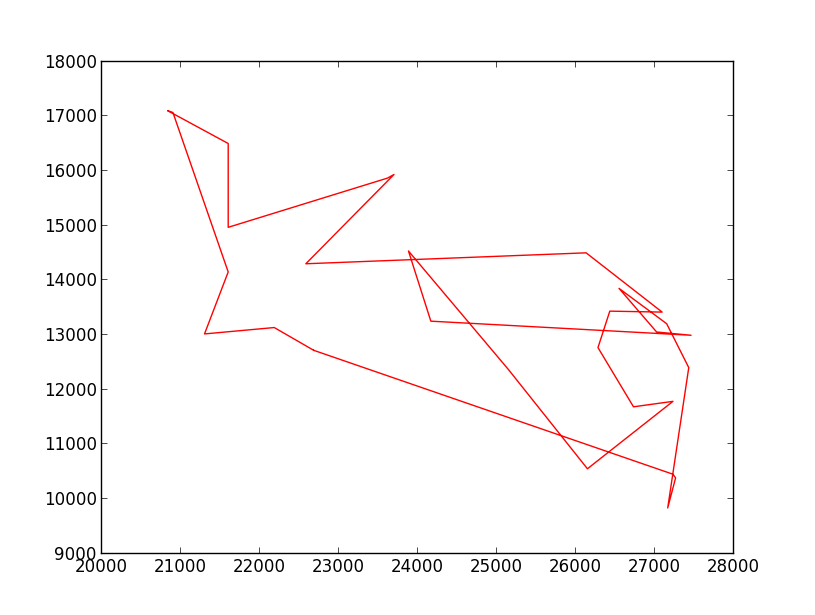
\includegraphics[width=7cm]{pmx1000.png} & 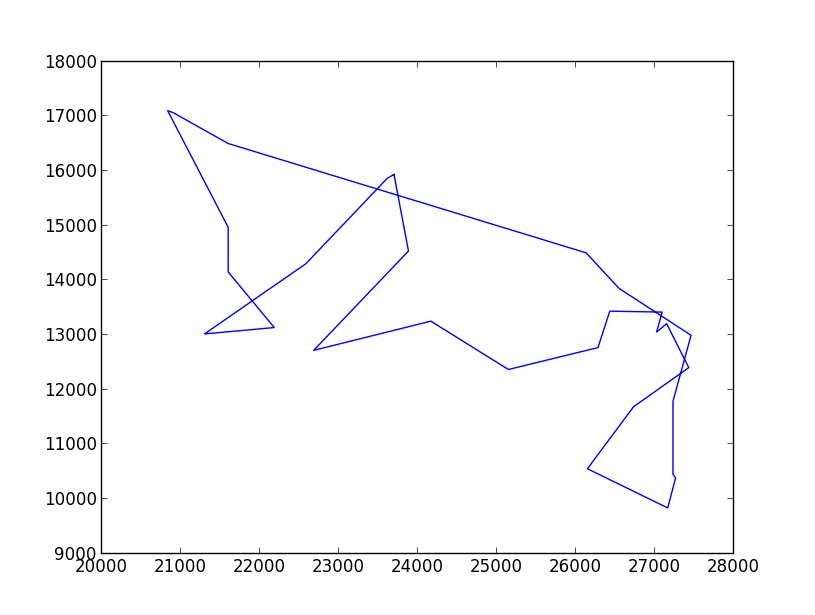
\includegraphics[width=7cm]{ox1000.png}
\end{tabular}



\end{document}